%%
%% Camera-ready submissions do not need line numbers, and
%% should have this option removed.
%%

\documentclass[fleqn,10pt,lineno]{manuscript}
%%\usepackage{setspace}
%%\doublespacing
\usepackage{soul}
\usepackage{xurl}
\usepackage{subcaption}
\newcommand{\beginsupplement}{%
        \setcounter{table}{0}
        \renewcommand{\thetable}{S\arabic{table}}%
        \setcounter{figure}{0}
        \renewcommand{\thefigure}{S\arabic{figure}}%
     }

\title{CDK4/6 inhibitors and endocrine therapy in the treatment of metastatic cancer: A real-world and Propensity Score-Adjusted comparison}

\author[1,2]{João Coutinho-Almeida}
\author[4]{Ana Sofia Silva}
\author[4]{Patricia Redondo}
\author[4]{Ana Ferreira}
\author[1,2,3]{Pedro Pereira Rodrigues}

\affil[1]{CINTESIS - Centre for Health Technologies and Services Research, University of Porto, Portugal}
\affil[2]{MEDCIDS – Faculty of Medicine of University of Porto, Portugal}
\affil[3]{Health Data Science PhD Program, Faculty of Medicine of the University of Porto, Portugal}
\affil[4]{IPO Porto, Portugal}

\corrauthor[1]{João Coutinho-Almeida}{joaofilipe90@gmail.com}

\keywords{Palbociclib; Ribociclib; Breast cancer; propensity score; real-world data; CDK4/6}

\begin{abstract}

\end{abstract}

\begin{document}

\flushbottom
\maketitle
\thispagestyle{empty}


\section*{Introduction}
Currently, metastatic breast cancer is difficult to treat. Patients with Hormone Receptor-positive (HR+) and Human Epidermal Growth Factor Receptor 2-negative (HER2-) breast cancer, the most common subtype, typically undergo endocrine therapy. Therefore, new treatments can be very useful in improving quality of life, reducing toxicity, and decreasing scenarios of hormonal resistance.
Medications from the group of cyclin-dependent kinase inhibitors appear as a potential improvement in the therapeutic approach to advanced breast cancer. Within this group, there are palbociclib, ribociclib, and abemaciclib. Cyclin-dependent kinases 4 and 6 $($CDK4/6$)$ are responsible for regulating the cell cycle at the transition between the G1 and S phases. In many neoplasms, this cycle is deregulated, and it promotes uncontrolled cell proliferation. It is then possible for these medications to have better effectiveness. These medications were approved by INFARMED, I.P. after an analysis of the therapeutic value they offer. For this purpose, data from clinical trials conducted with these medications were essentially used. The MONALEESA \cite{hortobagyiUpdatedResultsMONALEESA22018, slamonPhaseIIIRandomized2018, tripathyRibociclibEndocrineTherapy2018} studies were used for ribociclib, PALOMA \cite{vermaPalbociclibCombinationFulvestrant2016, rugoImpactPalbociclibLetrozole2018, finnCyclindependentKinaseInhibitor2015a} for palbociclib, and MONARCH \cite{goetzMONARCHAbemaciclibInitial2017, sledgeMONARCHAbemaciclibCombination2017} for abemaciclib.
These studies focused on testing the hypothesis of treating CDK4/6 inhibitors in combination with an aromatase inhibitor or fulvestrant as an alternative to the gold standard. In these studies, it was concluded that they brought a significant increase in effectiveness, justifying their use in clinical practice.
However, this evaluation was based on clinical trials with very specific inclusion and exclusion criteria and in a highly controlled environment. It is then vital to study how these new molecules compare to current practice in terms of treatment effectiveness in a real-world setting. In the meticulously controlled setting of clinical trials, patient selection often skews towards relatively healthier individuals with fewer comorbidities. However, in real-world clinical practice, patients present a diverse range of health profiles, co-existing illnesses, and medication histories that may influence drug efficacy and safety. Real-world data, drawn from electronic health records, insurance claims databases, and patient registries, offers the advantage of reflecting a more heterogeneous patient population, thus potentially uncovering insights not readily apparent in clinical trial settings. Understanding the effectiveness and safety of CDK4/6 inhibitors in real-world conditions is crucial for tailoring more individualized treatment regimens, optimizing outcomes, and enhancing quality of life for patients with HR+, HER2- breast cancer \cite{harbeckCDK4InhibitorsHR2021}. Nevertheless, observational studies have inherent limitations, such as confounding by indication, which can lead to biased estimates of treatment effects. To tackle this, there are causality-based assessments that can be employed in order to better estimate the causal effects of treatments.
Incorporating statistical techniques like Inverse Probability of Treatment Weighting (IPTW) can play an essential role in enhancing the quality of real-world evidence by accounting for treatment selection bias and balancing observed covariates between treatment groups. IPTW, grounded in the framework of causal inference, allows for the mimicking of a randomized control trial-like setting within observational studies. By assigning weights to individual patients based on their propensity scores—the likelihood of receiving a particular treatment given a set of observed characteristics—analyses can achieve balance between different treatment arms, thereby reducing bias and confounding factors. Establishing causality, rather than mere association, is vital for the robust interpretation of real-world data. As we strive to understand the long-term impact, efficacy, and safety of CDK4/6 inhibitors in HR+, HER2- breast cancer, the rigorous application of IPTW and causal inference methods can substantially augment the validity of real-world findings, making them a more reliable basis for clinical decision-making \cite{austinIntroductionPropensityScore2011,austinUsePropensityScore2014}
So in this paper, we propose:
\begin{itemize}
    \item To compare the effectiveness of the CDK4/6 inhibitors drug class in terms of PFS and OS.
\item Asess the Hazard Ratio of using the CDK4/6 inhibitors drug class in terms of PFS and OS.
    \item To compare the effectiveness of CDK4/6 inhibitors in combination with an aromatase inhibitor or fulvestrant with the current standard of care in terms of progression-free survival $($PFS$)$ and overall survival $($OS$)$ in patients with HR+, HER2- advanced breast cancer.
    \item assess the differences in effectiveness between the three CDK4/6 inhibitors in combination with an aromatase inhibitor or fulvestrant in terms of PFS and OS with causality principles in mind, especially the counterfactual theory and IPTW ;
\end{itemize}


%%%%%%%%%%%%%%%%%%%%%%%%%%%%%%%%%%%%%%%%%%
\section*{Materials and Methods}


\subsection{Study Design}

%This prospective study was designed in 2015 when palbociclib was approved by the National Administration of Medicines—ANMAT (Administración Nacional de Medicamentos, Alimentos y Tecnología Médica). The aim of the study was to evaluate the clinical benefit, side effects and long-term survival of patients with HR+/HER2− ABC treated with palbociclib plus ET in different lines of treatment between October 2015 and August 2019. Inclusion criteria: pre and postmenopausal women, men, Oestrogen Receptor positive (defined by ER expression ≥1% of tumour cell by immunohistochemistry, IHC) and HER2 negative (by IHC and/or amplification assay) in primary tumour or metastatic site after biopsy, that have received at least one cycle of palbociclib in advanced setting. 

This retrospective study was designed in 2022. The aim of the study was to evaluate the clinical benefit and long-term survival of patients with HR+/HER2$-$ that started treatment with CDK4\/6 inhibitors plus hormonotherapy in different lines of treatment between the 14th of March 2017 and the 31st of December 2021. The follow-up period was set until June 2022. 
Inclusion criteria:  postmenopausal women, men, Oestrogen Receptor positive \% (defined by ER expression $\geq$ 1 \% of tumour cell by immunohistochemistry, IHC)
and HER2 negative (by IHC and/or amplification assay) in the primary tumour or metastatic site after biopsy.
Exclusion criteria: Patients that had only ambulatory medication, and patients involved in clinical trials, diagnosed with other neoplasms or with active treatment during the study period.
The comparison group was defined by a population of patients, that were treated with hormone therapy as first-line (due to bone metastases) between 2015 and 13 of match 2017.

The evaluation of effectiveness will involve overall survival and progression-free analysis. We will compare the three different cyclin-dependent kinase inhibitors in terms of efficacy in real-world patients and will also compare the effectiveness of this class of drug against traditional hormonotherapy. 


%Desenho estudo
%Estudo cohort retrospetivo de RWD. Este estudo não implica qualquer alteração na prática clínica e nos procedimentos atualmente em vigor no IPO Porto para estes doentes.

%População
%Mulheres com neoplasia maligna da mama localmente avançada ou metastática, RH positivos, HER2 negativo, com indicação para tratamento com palbociclib, ribococlib ou abemaciclib, em associação com hormonoterapia.

%Critérios de inclusão:
%- Grupo de estudo: Doentes com neoplasia maligna da mama localmente avançada ou metastática, RH positivos, HER2 negativo, com indicação para tratamento com palbociclib, ribococlib ou abemaciclib, em associação com hormonoterapia, que iniciaram tratamento no IPO Porto (14/3/2017) até 31/12/2021;
%- Grupo controlo: Doentes que fizeram hormoterapia de 1ª linha (por metastização óssea) entre 2015 e 13/03/2017 (1º doente que iniciou inibidores das ciclinas).

%Critérios de exclusão:
%•	Doentes só com um levantamento na farmácia de ambulatório;
%•	Doentes com outras neoplasias diagnosticadas ou em tratamento ativo durante o período de estudo;
%•	Inclusão em ensaio clínico;
%•	Não realizar tratamento completo no IPO Porto.
 
%O período de follow up será até junho/2022.

%All data were collected from original medical records from baseline to last visit or death. Data included: demographic information, age at first diagnosis and age at the beginning of treatment with palbociclib, clinical characteristics and performance status by Eastern Cooperative Oncology Group scale (ECOG). Treatment-related data: loco-regional and neo/adjuvant systemic treatment, number and type of treatments in advance setting before palbociclib, type of treatment beyond palbociclib progression, treatment strategy in premenopausal women (ovarian suppression / ovarian ablation, OS/OA), palliative radiation therapy before or during palbociclib treatment and partner of palbociclib in different lines. Metastatic data at the beginning of palbociclib: ‘de novo’ metastatic disease, site of metastases (bone, soft tissue, visceral, visceral and bone, central nervous system-CNS with or without other site), and metastatic site at palbociclib progression. Patients predisposition: side effects by frequency and grade (NCI-CTCAE version 4.0), starting dose and number of patients with dose interruption, delay, reduction or treatment discontinuation

\subsection{Data collection}
All data were collected from original medical records from baseline to last visit or death.
The data was collected from  Instituto Português de Oncologia – Porto (IPO-P).  table \ref{tab:stats_ipop_cdk} shows a comparison between the groups.
%%%copied
Data included for population treated with CDK4\/6 inhibitors plus hormonotherapy : demographic information, age at first diagnosis and age at the beginning of treatment, clinical characteristics and performance status by Eastern Cooperative Oncology Group scale (ECOG), treatment line and treatment schema -  CDK4\/6 inhibitor and hormonotherapy, stage of the cancer, site of metastases (bone, soft tissue, visceral, visceral and bone, central nervous system-CNS with or without another site).
%%%copied
Data included for population treated with hormonotherapy as first-line: demographic information, age at first diagnosis and age at the beginning of treatment, clinical characteristics and performance status by Eastern Cooperative Oncology Group scale (ECOG),  stage of the cancer.

For comparasion purposes, we used palbociclib and ribociclib since we had a small number of patients treated with abemaciclib (12). We also filtered by 1st line to assess the best treatment option.

 
\begin{table}
\caption{Descriptive statistics of cyclin-dependent kinase inhibitors group}
\centering
\label{tab:stats_ipop_cdk}

\begin{tabular}[t]{llll}
\toprule
  & Palbociclib & Ribociclib & Overall\\
\midrule
 & (N=247) & (N=106) & (N=353)\\
\addlinespace[0.3em]
\multicolumn{4}{l}{\textbf{Age at treatment start}}\\
\hspace{1em}Mean (SD) & 59.2 (11.7) & 58.2 (10.7) & 58.9 (11.4)\\
\hspace{1em}Median [Min, Max] & 60.0 [28.0, 84.0] & 58.0 [32.0, 79.0] & 59.0 [28.0, 84.0]\\
\addlinespace[0.3em]
\multicolumn{4}{l}{\textbf{Bone Only metastases}}\\
\hspace{1em}No & 161 (65.2\%) & 74 (69.8\%) & 235 (66.6\%)\\
\hspace{1em}Yes & 86 (34.8\%) & 32 (30.2\%) & 118 (33.4\%)\\
\addlinespace[0.3em]
\multicolumn{4}{l}{\textbf{Combination}}\\
\hspace{1em}Exemestane & 1 (0.4\%) & 0 (0\%) & 1 (0.3\%)\\
\hspace{1em}Fulvestrant & 180 (72.9\%) & 10 (9.4\%) & 190 (53.8\%)\\
\hspace{1em}Letrozol & 66 (26.7\%) & 96 (90.6\%) & 162 (45.9\%)\\
\addlinespace[0.3em]
\multicolumn{4}{l}{\textbf{Treatment Line}}\\
\hspace{1em}1st Line & 127 (51.4\%) & 98 (92.5\%) & 225 (63.7\%)\\
\hspace{1em}2nd+ Lines & 120 (48.6\%) & 8 (7.5\%) & 128 (36.3\%)\\
\addlinespace[0.3em]
\multicolumn{4}{l}{\textbf{Visceral metastasis}}\\
\hspace{1em}No & 122 (49.4\%) & 49 (46.2\%) & 171 (48.4\%)\\
\hspace{1em}Yes & 125 (50.6\%) & 57 (53.8\%) & 182 (51.6\%)\\
\addlinespace[0.3em]
\multicolumn{4}{l}{\textbf{Stage}}\\
\hspace{1em}I & 22 (8.9\%) & 7 (6.6\%) & 29 (8.2\%)\\
\hspace{1em}II & 75 (30.4\%) & 22 (20.8\%) & 97 (27.5\%)\\
\hspace{1em}III & 75 (30.4\%) & 18 (17.0\%) & 93 (26.3\%)\\
\hspace{1em}IV & 65 (26.3\%) & 46 (43.4\%) & 111 (31.4\%)\\
\hspace{1em}Missing & 10 (4.0\%) & 13 (12.3\%) & 23 (6.5\%)\\
\bottomrule
\end{tabular}

\end{table}


\begin{table}[]
\caption{Descriptive statistics of palbociclib and ribociclib (1st line) group vs hormonotherapy}
\centering

\label{tab:stats_ipop_control}

\begin{tabular}[t]{llll}
\toprule
  & ET & Palbociclib & Ribociclib\\
\midrule
 & (N=43) & (N=246) & (N=106)\\
\addlinespace[0.3em]
\multicolumn{4}{l}{\textbf{Age at treatment start}}\\
\hspace{1em}Mean (SD) & 60.1 (12.4) & 59.2 (11.7) & 58.2 (10.7)\\
\hspace{1em}Median [Min, Max] & 62.0 [34.0, 85.0] & 60.0 [28.0, 84.0] & 58.0 [32.0, 79.0]\\
\addlinespace[0.3em]
\multicolumn{4}{l}{\textbf{Bone Only metastases}}\\
\hspace{1em}No & NA & 161 (65 \%) & 74 (70 \%)\\
\hspace{1em}Yes & NA & 85 (35 \%) & 32 (30 \%)\\
\hspace{1em}Missing & 43 (100\%) & 0 (0\%) & 0 \vphantom{1} (0\%)\\
\addlinespace[0.3em]
\multicolumn{4}{l}{\textbf{Visceral metastasis}}\\
\hspace{1em}No & NA & 121 (49 \%) & 49 (46 \%)\\
\hspace{1em}Yes & NA & 125 (51 \%) & 57 (54 \%)\\
\hspace{1em}Missing & 43 (100\%) & 0 (0\%) & 0 (0\%)\\
\addlinespace[0.3em]
\multicolumn{4}{l}{\textbf{Stage}}\\
\hspace{1em}I & 3 (7 \%) & 22 (9 \%) & 7 (7 \%)\\
\hspace{1em}II & 20 (47 \%) & 75 (30 \%) & 22 (21 \%)\\
\hspace{1em}III & 11 (26 \%) & 74 (30 \%) & 18 (17 \%)\\
\hspace{1em}IV & 2 (5 \%) & 65 (26 \%) & 46 (43 \%)\\
\hspace{1em}Missing & 7 (16.3\%) & 10 (4.1\%) & 13 (12.3\%)\\
\addlinespace[0.3em]
\multicolumn{4}{l}{\textbf{Drug/Combination}}\\
\hspace{1em}Anastrozol & 3 (7 \%) & NA & NA\\
\hspace{1em}Exemestane & 4 (9 \%) & NA & NA\\
\hspace{1em}Fulvestrant & 5 (12 \%) & 180 (73 \%) & 10 (9 \%)\\
\hspace{1em}Letrozol & 31 (72 \%) & 66 (27 \%) & 96 (91 \%)\\
\bottomrule
\end{tabular}

\end{table}

\subsection{Statistical Analysis}
%copied
R was used for statistical analysis. Demographic, clinical characteristics and side effects were analysed using descriptive statistics (count, percentages and median/range). Kaplan–Meier test was used to determine the median PFS and OS in the entire population and subgroups. Log-rank test was used for comparisons of PFS and OS among different subgroups. Cox Regression was used to assess feature importance and impact. All statistical tests were two-sided, and the significance level was 0.05. 




%Pretende-se que os dados venham do Instituto Português de Oncologia – Porto (IPO-P). Pretende-se utilizar a base de dados do hospital dos últimos 5 anos.
%O estudo será registado e respeitará todos os requisitos éticos de aprovação a comissão de ética de cada instituição participante. Caso a instituição tenha um encarregado de Proteção de Dados (EPD), este será contactado a fim de dar seu parecer, e caso necessário, a sua opinião para melhorar possíveis pontos relacionados à segurança de dados.

%The goal is to identify the clinical or biological variables that have the most impact on a specific outcome. To achieve this, considering the statistical models found, we can model things in terms of time series or survival trees to group outcomes and the clusters found. With this, we can analyze the effectiveness of the clinical course, probabilities of recurrence, or survival rates by subgroup. These models and relationships can form the basis of a clinical decision support system and can be crucial for making better healthcare decisions.

%Some of the techniques used are unsupervised techniques such as k-means, DBSCAN, or hierarchical clustering.
%The goal is to identify the clinical or biological variables that have the most impact on a specific outcome. To achieve this, considering the statistical models found, we can model things in terms of time series or survival trees to group outcomes and the clusters found. With this, we can analyze the effectiveness of the clinical course, probabilities of recurrence, or survival rates by subgroup. These models and relationships can form the basis of a clinical decision support system and can be crucial for making better healthcare decisions.

%Some of the techniques used are unsupervised techniques such as k-means, DBSCAN, or hierarchical clustering.




% breast cancer cells have either estrogen (ER) or progesterone (PR) receptors or both. (HR +)

%%%%%%%%%%%%%%%%%%%%%%%%%%%%%%%%%%%%%%%%%%
\section*{Results}


%\begin{figure}[ht]
%\caption{Clustering for 3 variables with 3 silos - (A) categorical variables with  proportion with K-Means and (B)  Categorical with K-modes  }\label{fig:interest} 
%  \subcaptionbox*{(A)}[.44\linewidth]{%
%    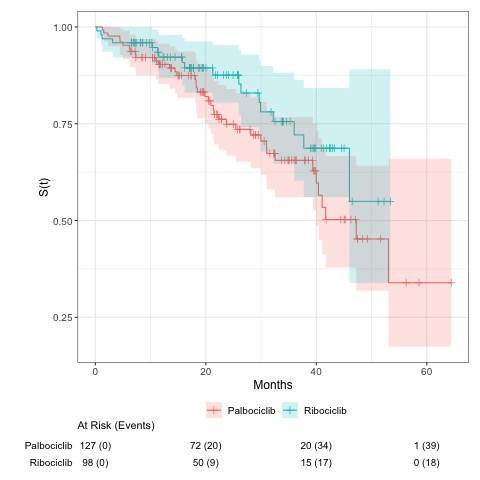
\includegraphics[width=\linewidth]{figures/interest_curve_OS.jpeg}%
%  }%
%  \hfill
%  \subcaptionbox*{(B)}[.44\linewidth]{%
%    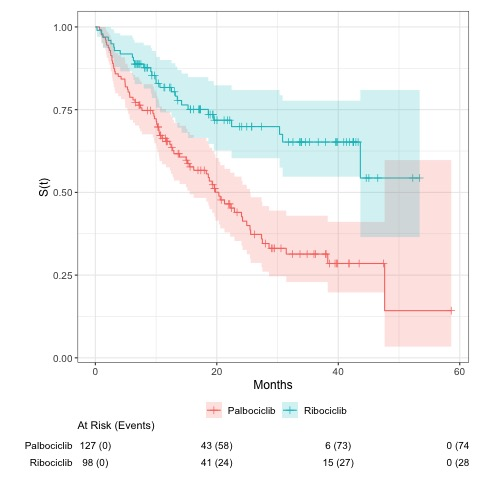
\includegraphics[width=\linewidth]{figures/interest_curve_PFS.jpeg}%
%  }
%\end{figure}

\begin{figure}[ht]
  \caption{Survival curves for Palbociclib and Ribociclib - Progression Free Survival and Overall Survival}\label{fig:interest} 
  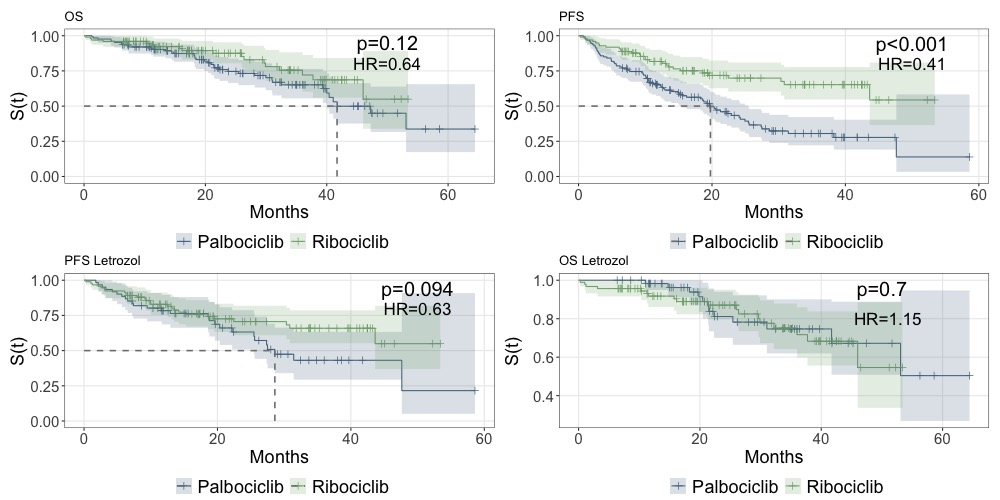
\includegraphics[scale=0.4]{figures/interest_curve_both.jpeg}%

\end{figure}


\begin{figure}[ht]
  \centering
  \caption{Cox Regression with palbociclib and Ribociclib - Progression Free Survival and Overall Survival}\label{fig:cox} 
  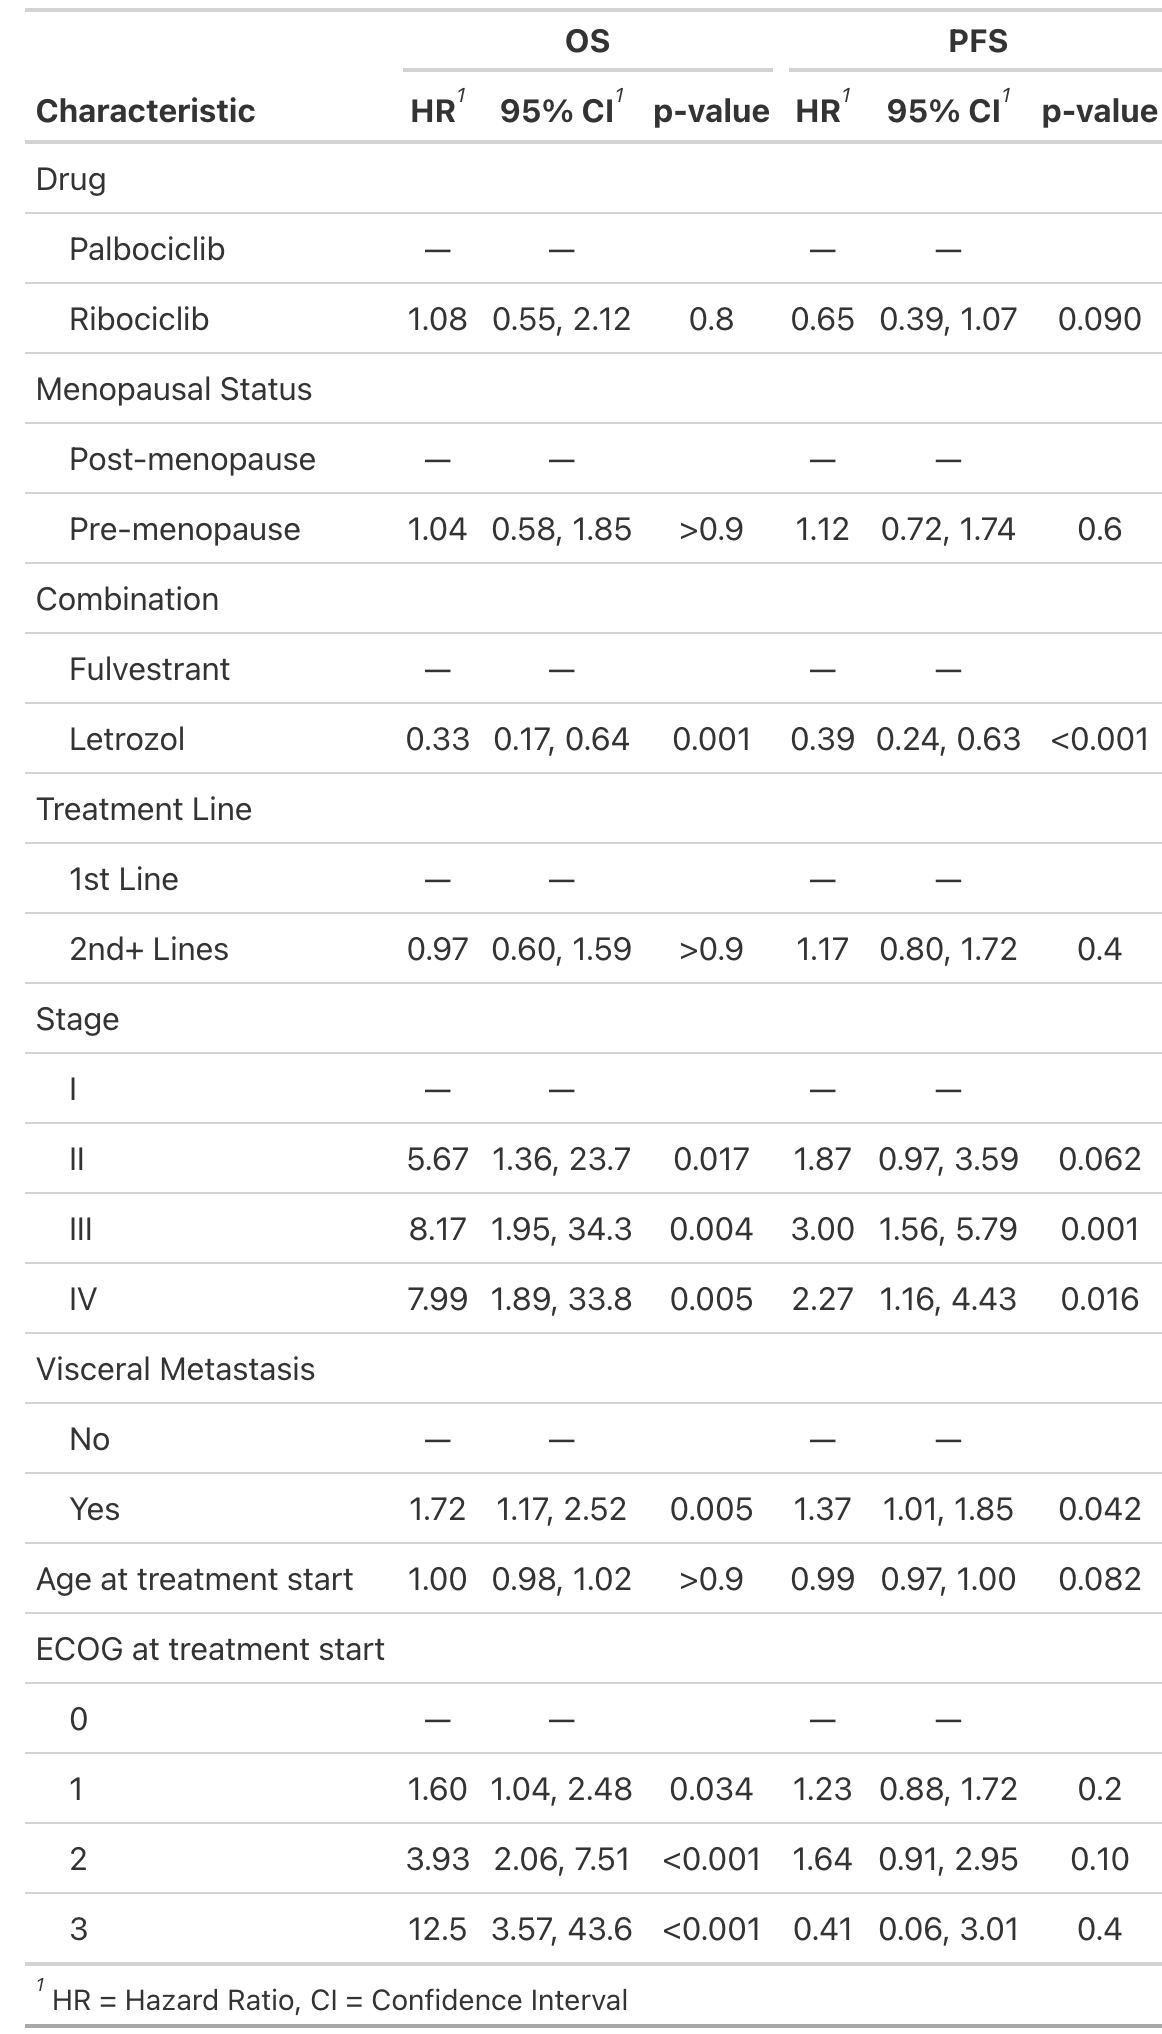
\includegraphics[scale=0.3]{figures/cox_both.png}%

\end{figure}

\begin{figure}[ht]
  \centering

  \caption{Comparision of traditional hormonotherapy and CDK4/6 inhibitors  }\label{fig:grouped} 
  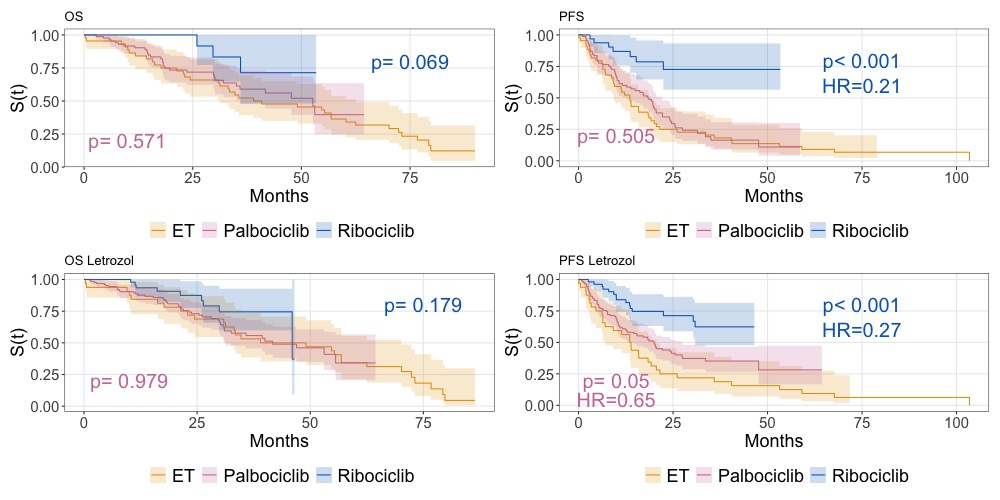
\includegraphics[scale=0.4]{figures/grouped_curve_both.jpeg}%

\end{figure}

\begin{figure}[ht]
  \centering

  \caption{Comparasion of palbociclib and ribociclib adjusted for propensity scores  }\label{fig:propensity} 
  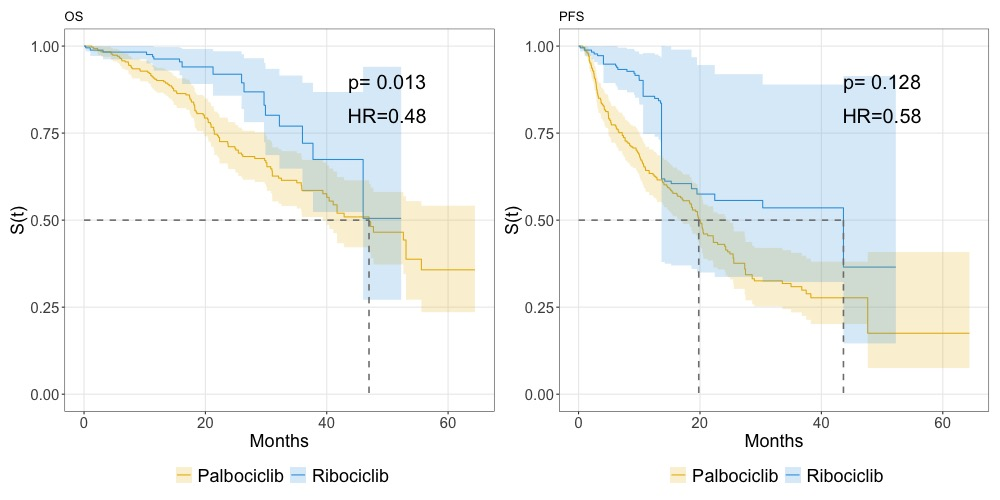
\includegraphics[scale=0.35]{figures/propensity_score_both.jpeg}%

\end{figure}


 
%%%%%%%%%%%%%%%%%%%%%%%%%%%%%%%%%%%%%%%%%%
\section*{Discussion}
This study aimed to evaluate the real-world use of palbociclib and ribociclib in combination with ET for HR+/HER2- and compare this drug class with traditional endocrine therapy. Few real-world evidence studies of palbociclib and ribociclib used in daily clinical practice have been published identifying clinical benefits, patient profiles, and sequencing of treatment, with even less evidence for the Portuguese population.

When comparing with clinical trials, regarding patient profile, in our study, 51\% had visceral metastasis and 35\% had bone-only metastases compared with 49\% and 38\% in PALOMA-2, and 60\% and 25\% in PALOMA-3, respectively \cite{rugoImpactPalbociclibLetrozole2018,cristofanilliFulvestrantPalbociclibFulvestrant2016a}.
As for ribociclib and bone-only metastases, MONALEESA-7 \cite{tripathyRibociclibEndocrineTherapy2018} has 24\% and MONALEESA-2 has 40\% \cite{hortobagyiUpdatedResultsMONALEESA22018} and our study has 30\%.
Regarding menopausal status, our study has 20\% premenopausal and 80\% postmenopausal.


Of note, the range of median PFS for first-line palbociclib was 15.5–25.5 months, which is shorter than 27.6 months observed in a post hoc analysis of the PALOMA-2 clinical trial with extended follow-up \cite{rugoImpactPalbociclibLetrozole2018}, but in line with RWE studies (13.3–20.2 months) \cite{harbeckCDK4InhibitorsHR2021}. When assessed with only letrozoleas a combination, the median PFS increased to 28.6 months [95\% CI 25.5-not reached].
Additionally, analyzing the postmenopausal women subgroup, palbociclib showed a median PFS of 16.3 months [95\% CI 12.9 -20]. Furthering analysis of the postmenopausal and with letrozole, the median was 47.6 months [95\% 25.6-2–not reached].

As for ribociclib, median survival time was not reached whether in OS and PFS. So we can at least say that the median PFS is longer than 50 months. This is longer than the median progression-free survival of 23.8 months (95\% CI 19.2–not reached) reported in the MONALEESA-7 trial \cite{tripathyRibociclibEndocrineTherapy2018} and longer than  25.3 months (95\% CI 23.0–30.3) in the MONALEESA-2 trial \cite{hortobagyiUpdatedResultsMONALEESA22018}. 
Regarding the subgroup analysis of postmenopausal women and postmenopausal women treated ribociclib in combination with letrozole, the median was not reached.

When directly comparing ribociclib and palbociclib without any adjustments, one might deduce that ribociclib is superior to palbociclib. However, after adjusting for confounding variables, there is no significant difference between the two inhibitors in terms of Progression-Free Survival (PFS) or Overall Survival (OS) as indicated in \ref*{tab:cox}. This observation is further corroborated by the lower plots in \ref*{fig:interest}, where even a subgroup analysis of CDK4/6i combined solely with letrozole reveals a trend towards nonsignificance.

In the first-line comparison between Endocrine Therapy (ET) and CDK4/6 inhibitors (CDK4/6i), there is no significant impact on Overall Survival (OS) by either treatment, whether the CDK4/6i is combined with both agents or solely with letrozole. With respect to Progression-Free Survival (PFS), ribociclib demonstrates superior efficacy in both combination therapies (HR=0.29) as well as when paired only with letrozole (HR=0.28). Additionally, palbociclib exhibits significant improvement in PFS when combined with letrozole (HR=0.50).

In the first-line comparison, the analysis of overall survival outcomes reveals no substantial difference between endocrine therapy alone and the combination of CDK4/6 inhibitors with endocrine therapy, irrespective of whether the CDK4/6 inhibitors are administered concomitantly with both fulvestrant and letrozole or exclusively with letrozole (figure 2 left). With respect to PFS, ribociclib demonstrates superior efficacy in both combination therapies (HR=0.21) as well as when paired only with letrozole (HR=0.27). Additionally, palbociclib exhibits significant improvement in PFS when combined with letrozole (HR=0.65) (figure 2 right).


When comparing with propensity scores weighting, we found out that ribociclib is significantly better than palbociclib for PFS and OS, providing a median OS of over 40 months and median PFS of around 42 months. Adjusted for the weighted variables, Ribociclib is not significantly better for PFS, but has a p-value of 0.013 for OS with an HR of 0.48. However, the Cox regression adjusted for variables and weights are not significant, even when the p-value for PFS is 0.05. This suggests that a more in depth analysis may be necessary.





%%%%%%%%%%%%%%%%%%%%%%%%%%%%%%%%%%%%%%%%%%
\section*{Conclusions}
In conclusion, our findings underscore the efficacy of CDK4/6 inhibitors in real-world settings. While we cannot definitively assert that palbociclib surpasses endocrine therapy in terms of Overall Survival—a facet not extensively explored in prominent clinical trials—we can confidently affirm the impact of CDK4/6i on Progression-Free Survival. This assertion aligns with clinical trial outcomes and real-world data further substantiates these findings.

Delving deeper into the characteristics of the patient population, including safety profiles, economic implications, and quality of life metrics, would be insightful. Additionally, a thorough examination of biomarkers within the population could offer invaluable insights. We intend to explore these facets in subsequent publications.

It's imperative to note that our data is sourced from a singular institution, limiting the generalizability of our results to a broader population. Nonetheless, we posit that this study lays a foundational groundwork for future research in this domain. While our evidence is rooted in observational data and we've made adjustments for known confounders, the potential for residual confounding remains. Although the use of propensity score matching enhances the comparative robustness between the groups, the presence of unmeasured confounders cannot be entirely ruled out. Furthermore, the small sample size of our study limits the statistical power of our findings. We hope that our study will serve as a springboard for future research in this domain, and we look forward to furthering our research in this area.



%%%%%%%%%%%%%%%%%%%%%%%%%%%%%%%%%%%%%%%%%%
\section*{Declarations}


\subsection*{Authors' contributions}

J.A., A.S., P.R. and A.F. conceived the idea; P.R. contributed to the experimental design and was in charge of overall direction and planning; All authors contributed to discussion and data analysis; J.A. wrote the main manuscript; All authors read and agreed to the published version of the manuscript.

\subsection*{Availability of data and materials}

The data is not publicly available due to privacy or ethical restrictions. The code is available at \url{}.

\subsection*{Acknowledgements}

...

\subsection*{Ethics approval and consent to participate}

This project was approved by the hospital ethics committee and privacy officers with the reference number CES 193/022. The need for informed consent was waived by the ethics committee.

\subsection*{Funding}

Not applicable

\subsection*{Competing interests}

Not applicable



%%%%%%%%%%%%%%%%%%%%%%%%%%%%%%%%%%%%%%%%%%
\bibliographystyle{plain}
\bibliography{main}


%%%%%%%%%%%%%%%%%%%%%%%%%%%%%%%%%%%%%%%%%%
\section*{Figure}


%%%%%%%%%%%%%%%%%%%%%%%%%%%%%%%%%%%%%%%%%%
\section*{Table}


%%%%%%%%%%%%%%%%%%%%%%%%%%%%%%%%%%%%%%%%%%
\clearpage

\beginsupplement
\renewcommand\figurename{Supplementary Figure}
\renewcommand\tablename{Supplementary Table}


\section*{Supplementary Material}


\end{document}
